\documentclass{exam}
\usepackage[exos]{main}

\title{Du nombre dérivé à la fonction dérivée}
\date{13 Mai 2025}
\author{Maths Spécifiques}

\begin{document}
\maketitle
\begin{questions}
\question Soit $f$ un fonction dont la courbe représentative $\mathcal{C}_f$ est donnée ci-après.
\begin{center}
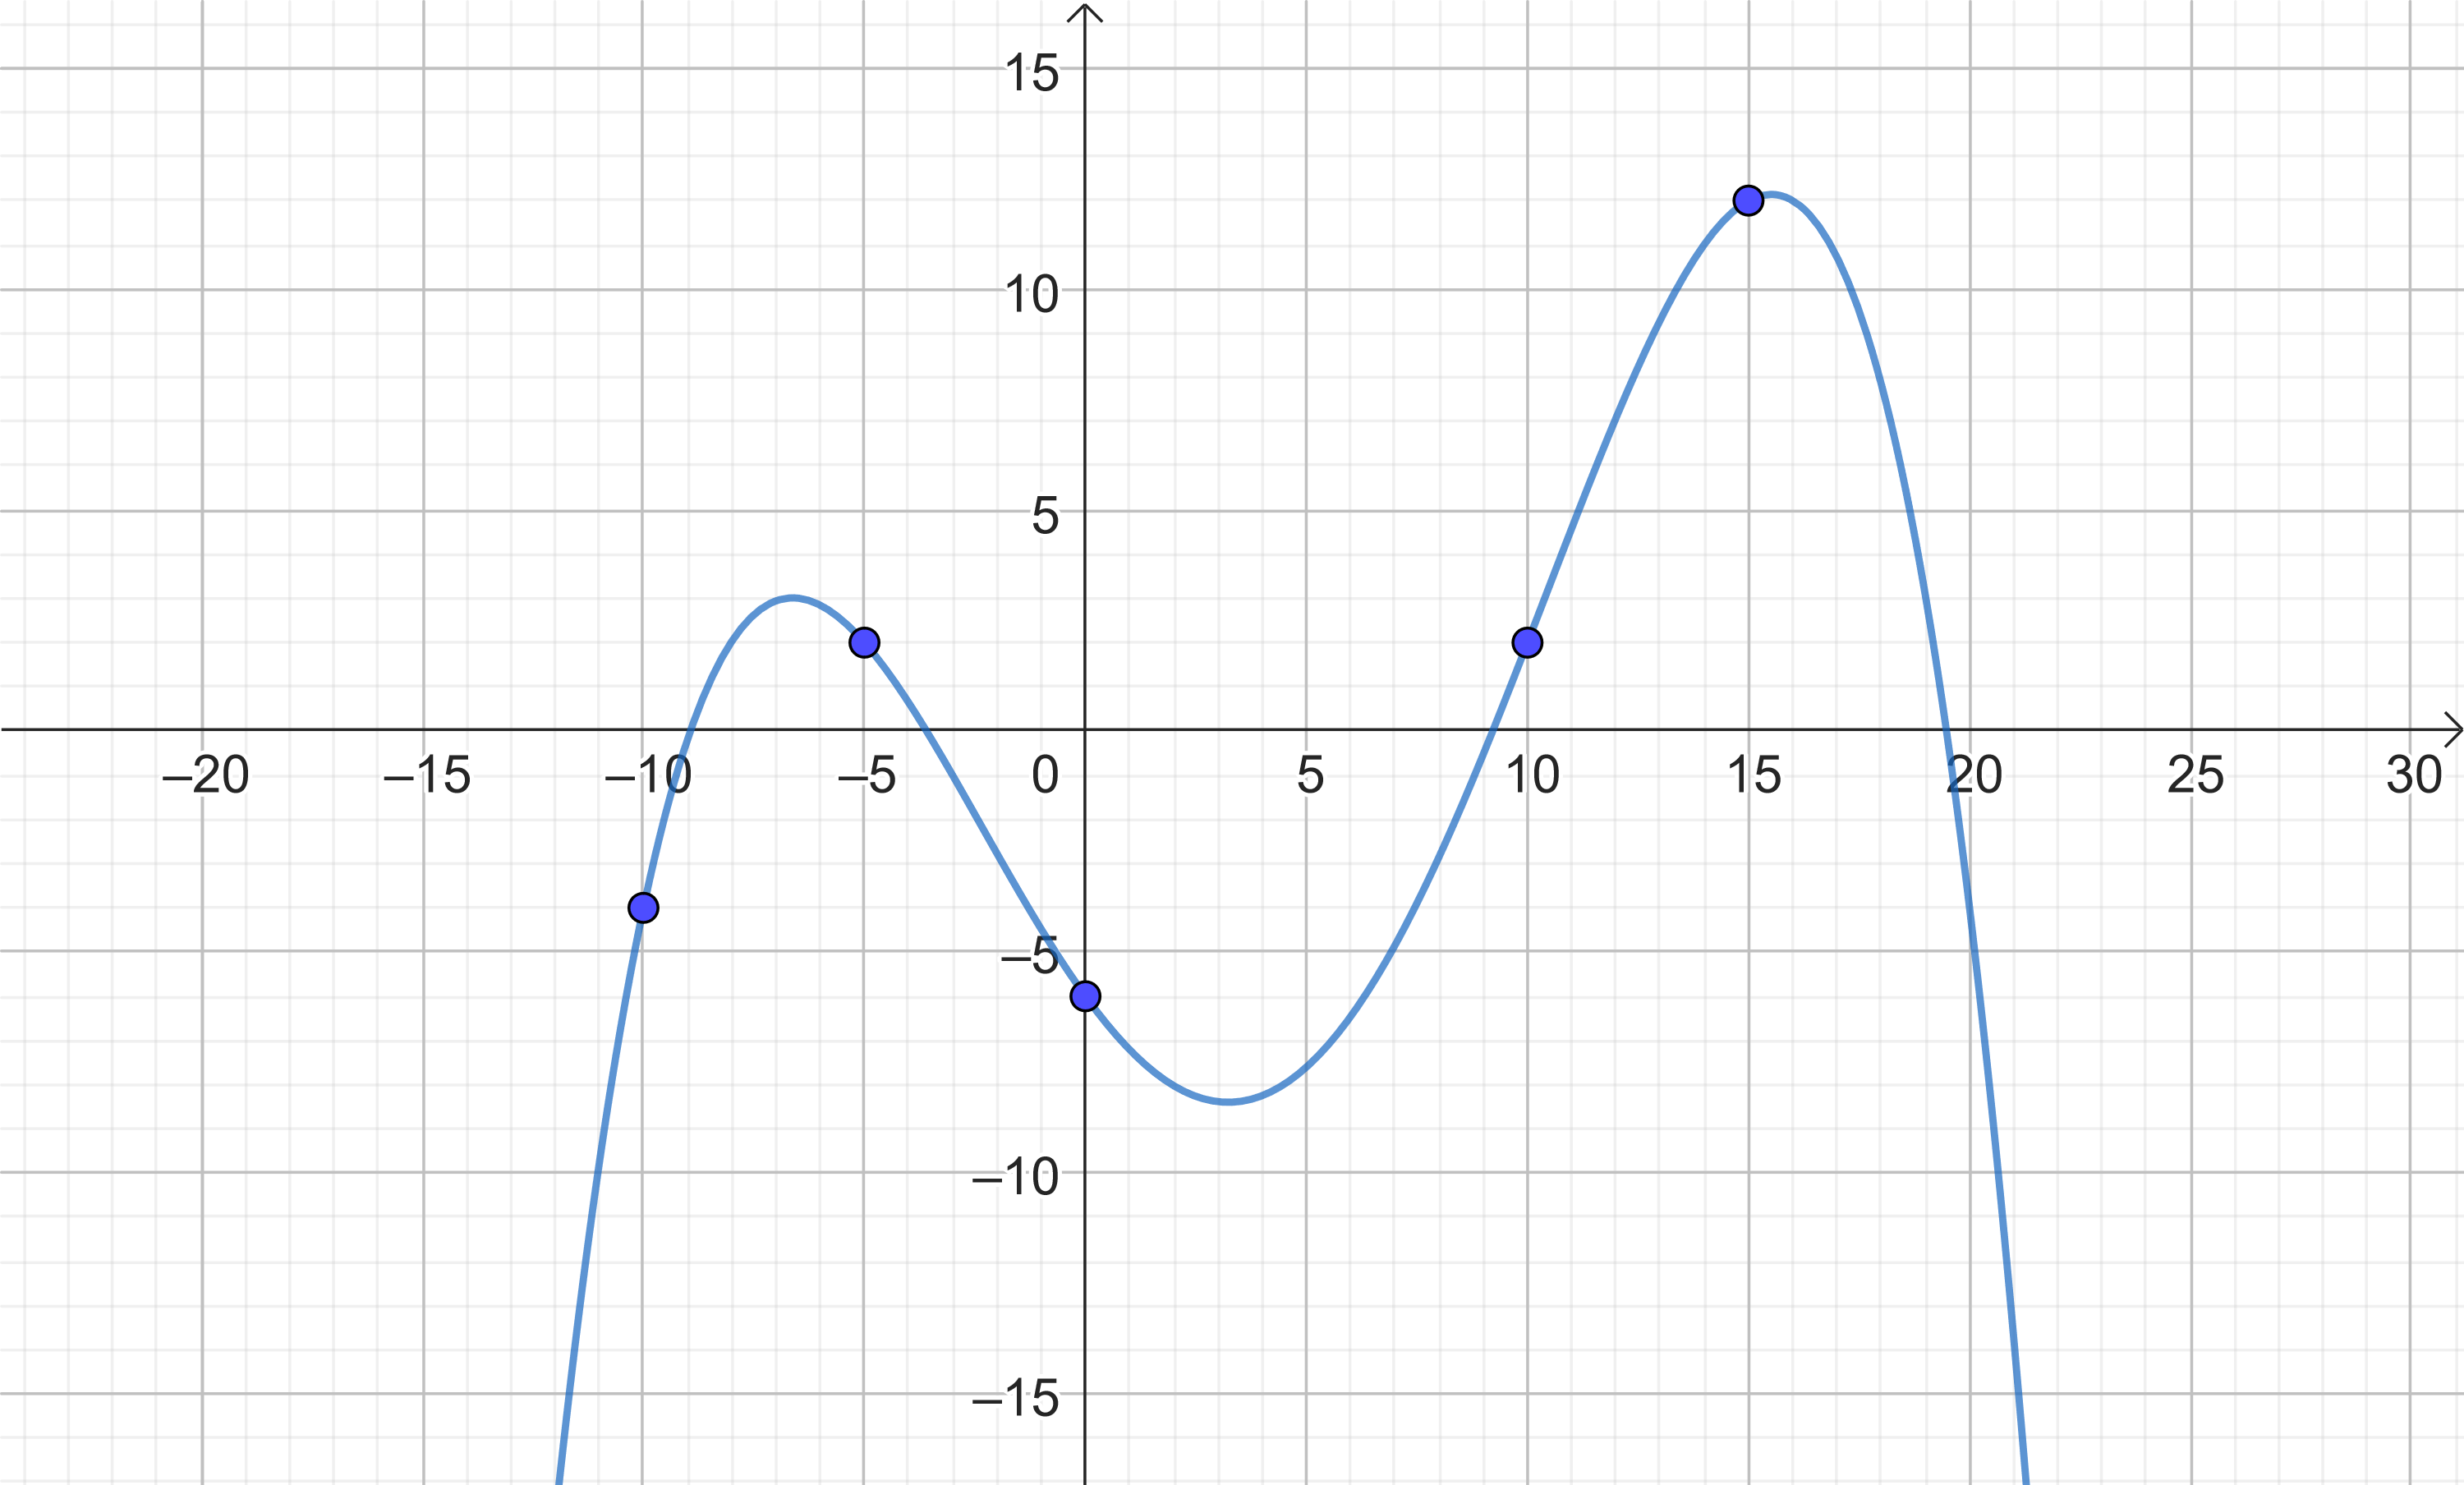
\includegraphics[width=0.9\textwidth]{13_05_2024.png}
\end{center}
\begin{parts}
\part Tracer les tangentes à $\mathcal{C}_f$ passant par $A(-10;f(-10))$, $B(-5;f(-5))$ et $C(15;f(15))$.
\part On note $f'(a)$ le nombre dérivé de $f$ en $a$. Trier par ordre croissant $f'(-10)$, $f'(-5)$ et $f'(15)$.
\part Tracer la tangente à $f$ en un nombre supérieur à $16$. Quel est le signe de son nombre dérivé ? Etait-ce prévisible ?
\end{parts}
\makeemptybox{7cm}
\newpage
\question
On souhaite étudier le nombre dérivé en $0$ de la fonction $f \colon x \mapsto \dfrac{1}{2}x + 1$.
\begin{parts}
\part Tracer la courbe représentative de $f$ sur le repère ci-contre.
\begin{center}
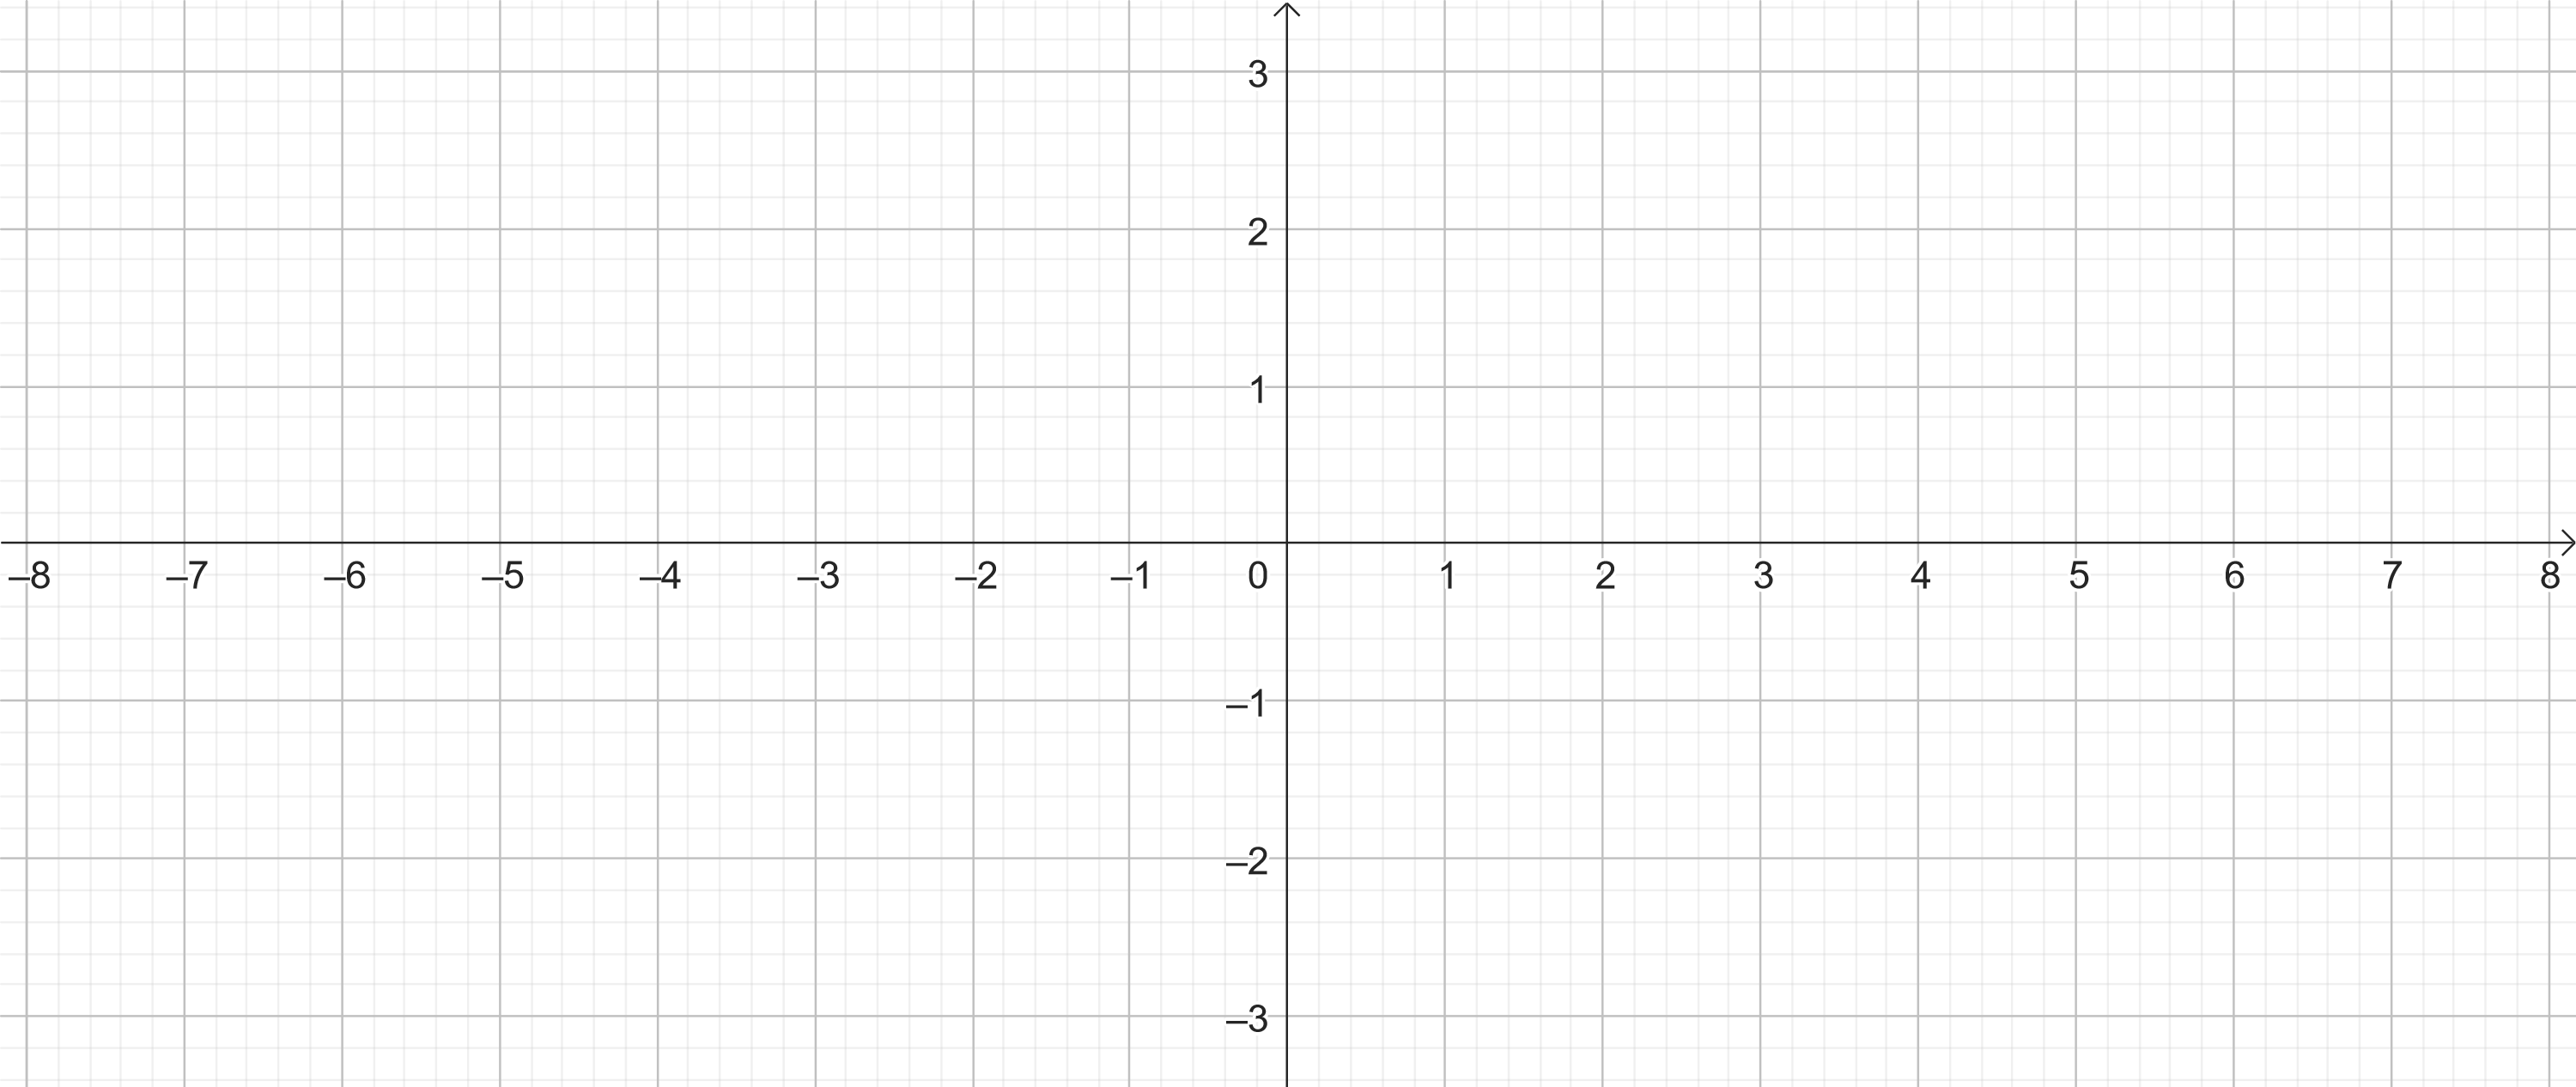
\includegraphics[width=0.9\textwidth]{13_05_2024_2.png}
\end{center}
\part Tracer la tangente à $\mathcal{C}_f$ passant par $A(0;f(0))$. En déduire le nombre dérivé de $f$ en $0$.
\part Une autre façon de calculer le nombre dérivé est de calculer des taux d'accroissement. Avec les valeurs de $x_1$ et de $x_2$ de votre choix, vérifier que le taux d'accroissement
\begin{equation*}
\dfrac{f(x_2)-f(x_1)}{x_2-x_1}
\end{equation*}
vaut bien $\dfrac{1}{2}$.
\part L'affirmation suivante est-elle vraie ? 
\begin{tcolorbox}
Pour tout $a$, le nombre dérivé de $f$ en $a$ est $\dfrac{1}{2}$
\end{tcolorbox}
\end{parts}
\makeemptybox{4cm}
\question On cherche le nombre dérivé de $f \colon x \mapsto x^2$ en $a=0$. Pour ce faire, on prend $h > 0$.
\begin{parts}
\part Calculer le taux d'accroissement de $f$ entre $a$ et $a+h$.
\part Vers quoi tend ce taux d'accroissement si $h$ tend vers $0$ ? En déduire le nombre dérivé de $f$ en $0$.
\part Même question pour $a=1$.
\end{parts}
\makeemptybox{4cm}
\end{questions}
\end{document}
